% Homework 16.tex 

\documentclass{article}
\usepackage{graphicx} % for figures
\usepackage{float}
\usepackage[export]{adjustbox}
\usepackage{fancyhdr}
\begin{document}

\title{Homework 11 - Physics 240\\
		Fourier Analysis}
\author{Tin Tran}

\maketitle

\section{Introduction}
The goal of this homework is to apply the Fourier transformation to some waves to calculate their spectrum.

\section{Discussion and data}
I have modified the code to take user input for the function, the number of data points, and the frequency. So you can run the program with all the parameters and it will plot out all the combinations all at once, or stop when you tell it to stop.\\
*Because of the time limit I can only include a few plots here(one case of Fs and N), but the code will plot any user input of the number of data points and frequency.

\begin{figure}[H]
\centering{
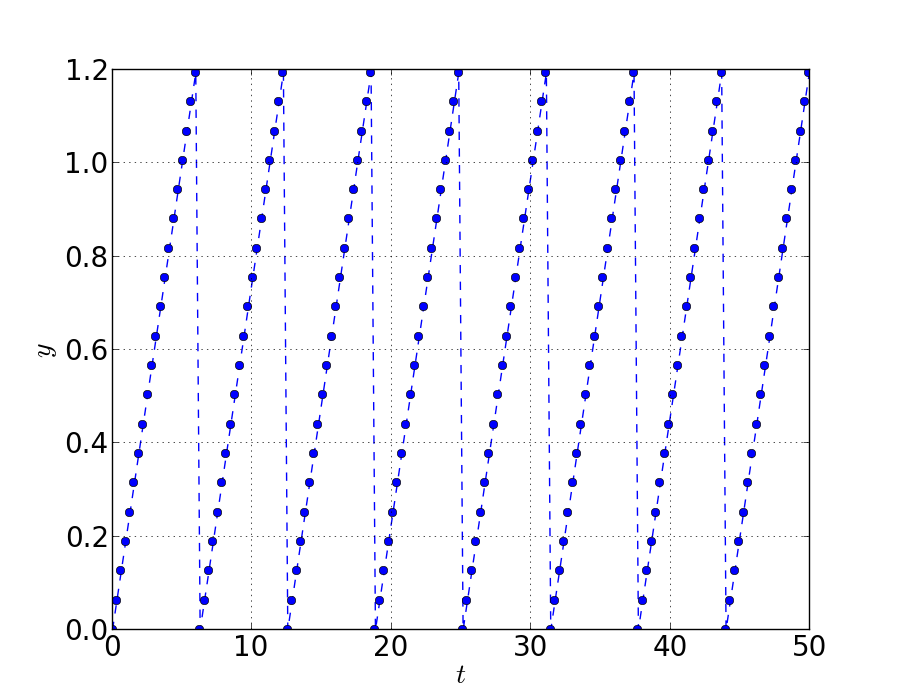
\includegraphics[max size={3 in}{4 in}]{a1.png}
\caption{}
}
\end{figure}

\begin{figure}[H]
\centering{
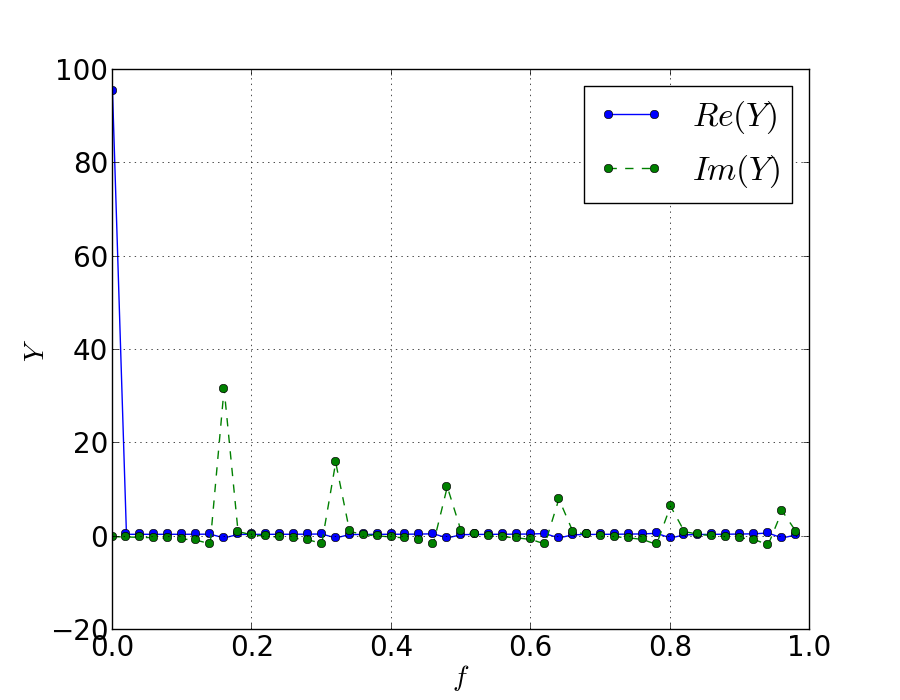
\includegraphics[max size={3 in}{4 in}]{a2.png}
\caption{}
}
\end{figure}

\begin{figure}[H]
\centering{
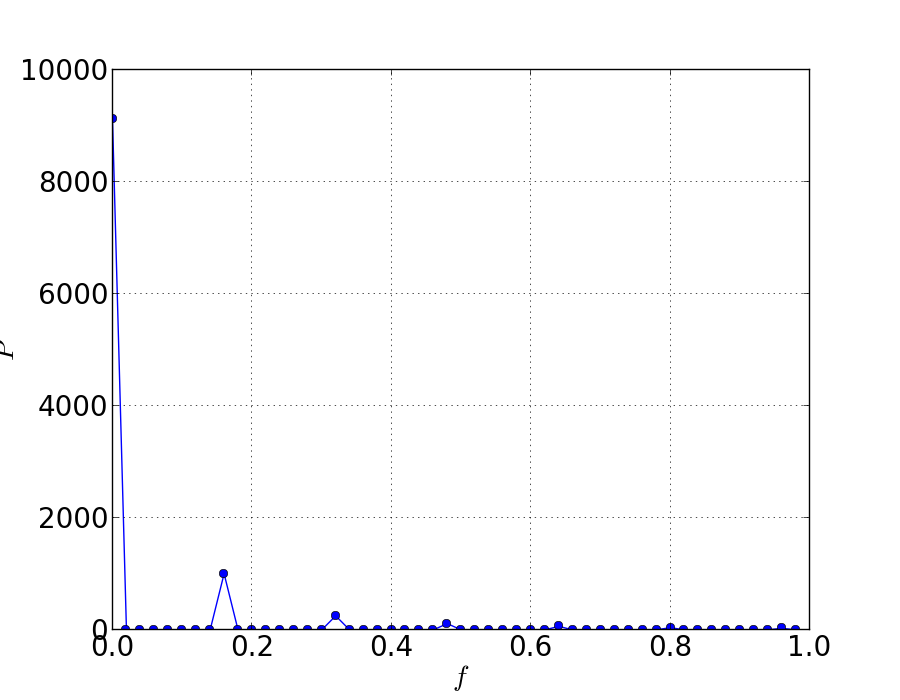
\includegraphics[max size={3 in}{4 in}]{a3.png}
\caption{}
}
\end{figure}

\begin{figure}[H]
\centering{
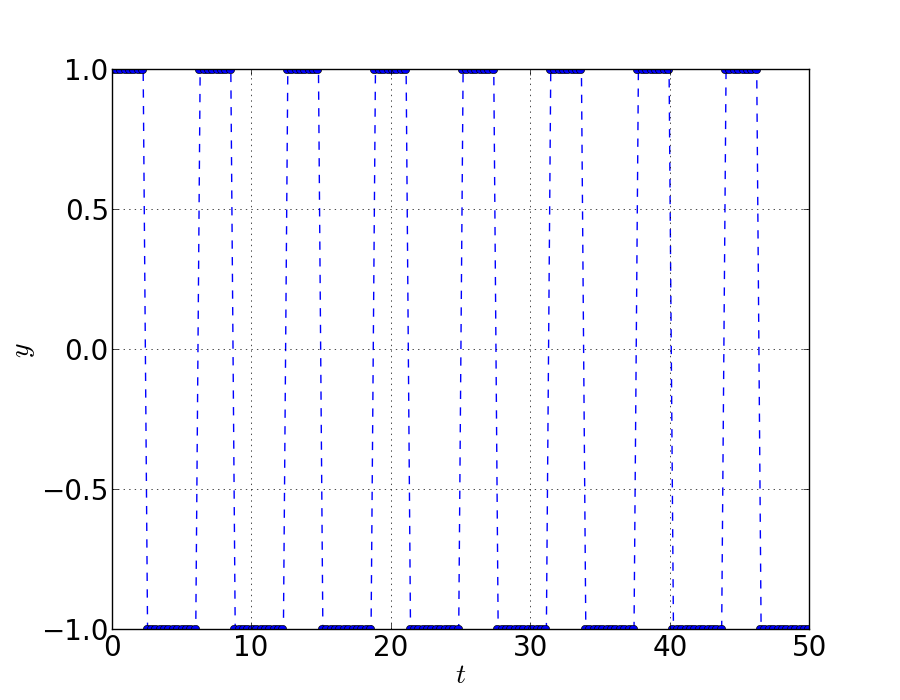
\includegraphics[max size={3 in}{4 in}]{b1.png}
\caption{}
}
\end{figure}
\begin{figure}[H]
\centering{
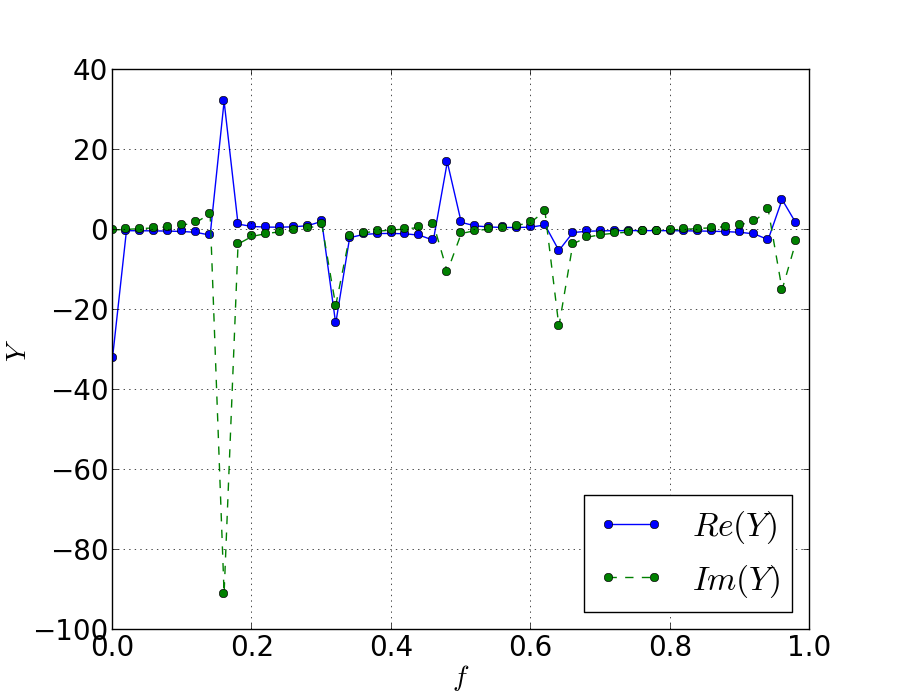
\includegraphics[max size={3 in}{4 in}]{b2.png}
\caption{}
}
\end{figure}
\begin{figure}[H]
\centering{
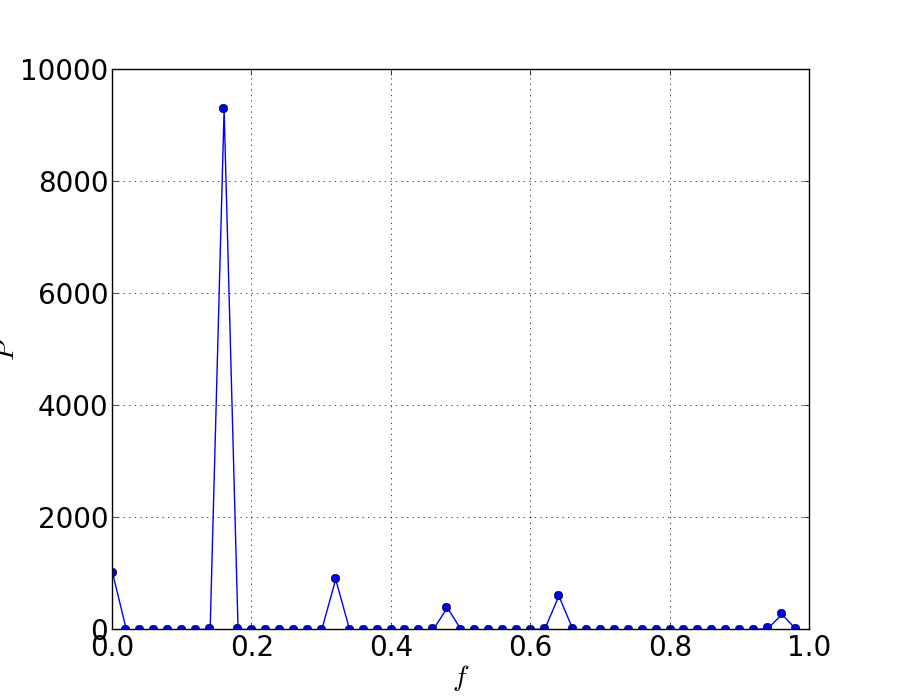
\includegraphics[max size={3 in}{4 in}]{b3.png}
\caption{}
}
\end{figure}

\begin{figure}[H]
\centering{
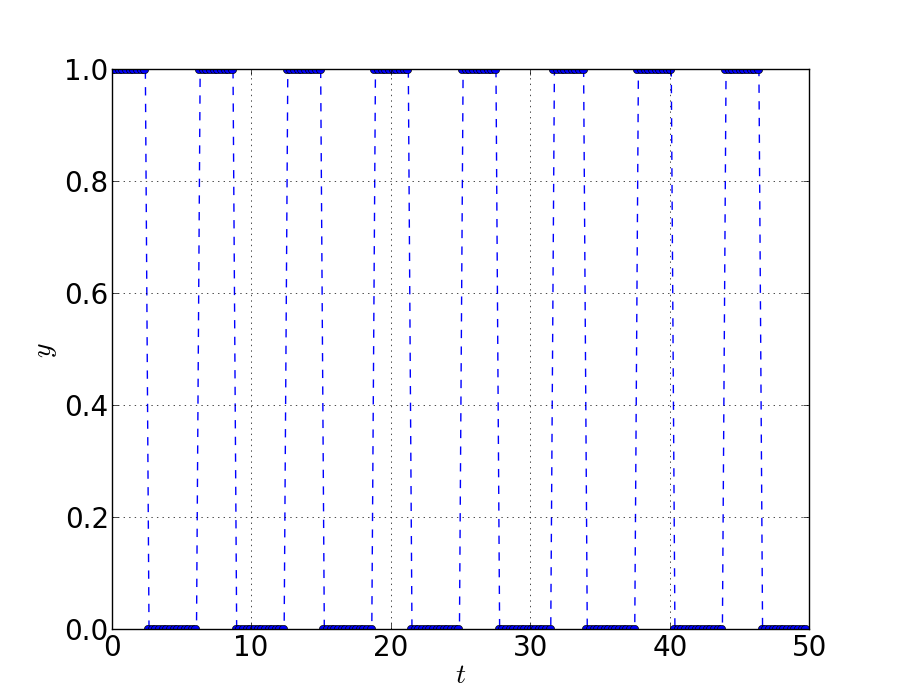
\includegraphics[max size={3 in}{4 in}]{c1.png}
\caption{}
}
\end{figure}

\begin{figure}[H]
\centering{
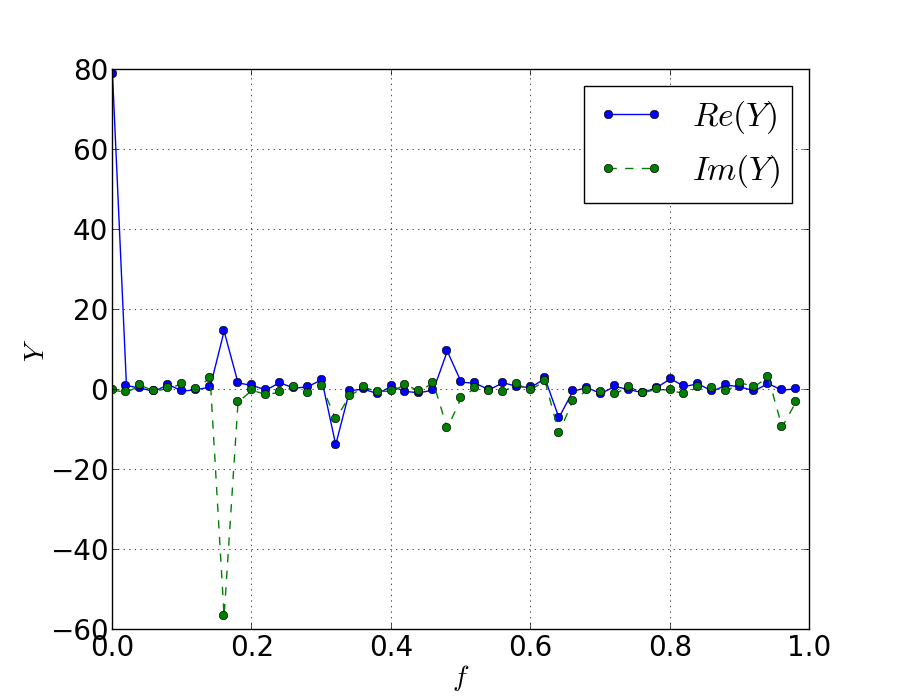
\includegraphics[max size={3 in}{4 in}]{c2.png}
\caption{}
}
\end{figure}

\begin{figure}[H]
\centering{
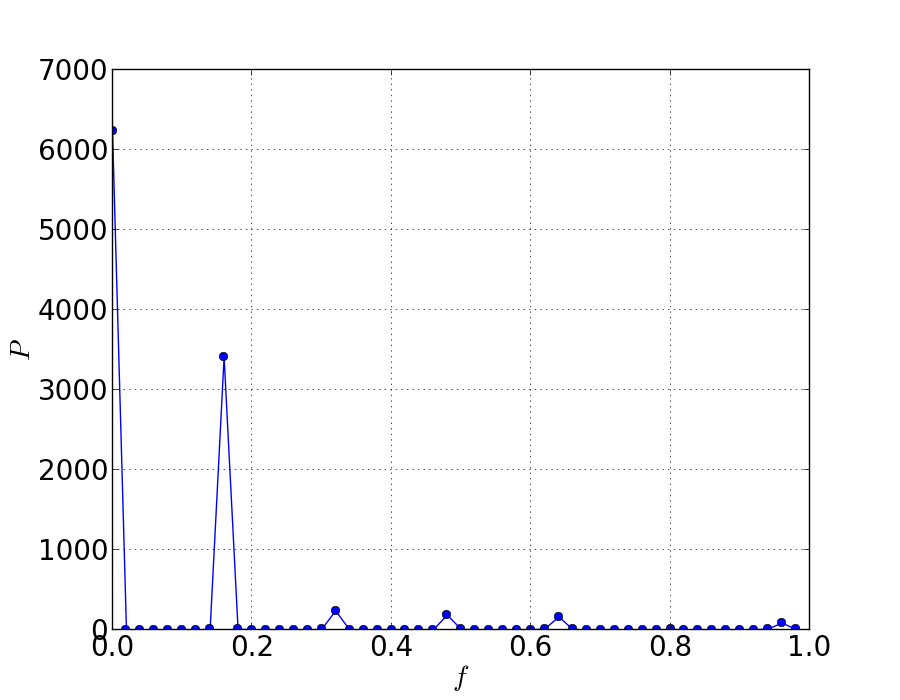
\includegraphics[max size={3 in}{4 in}]{c3.png}
\caption{}
}
\end{figure}

\begin{figure}[H]
\centering{
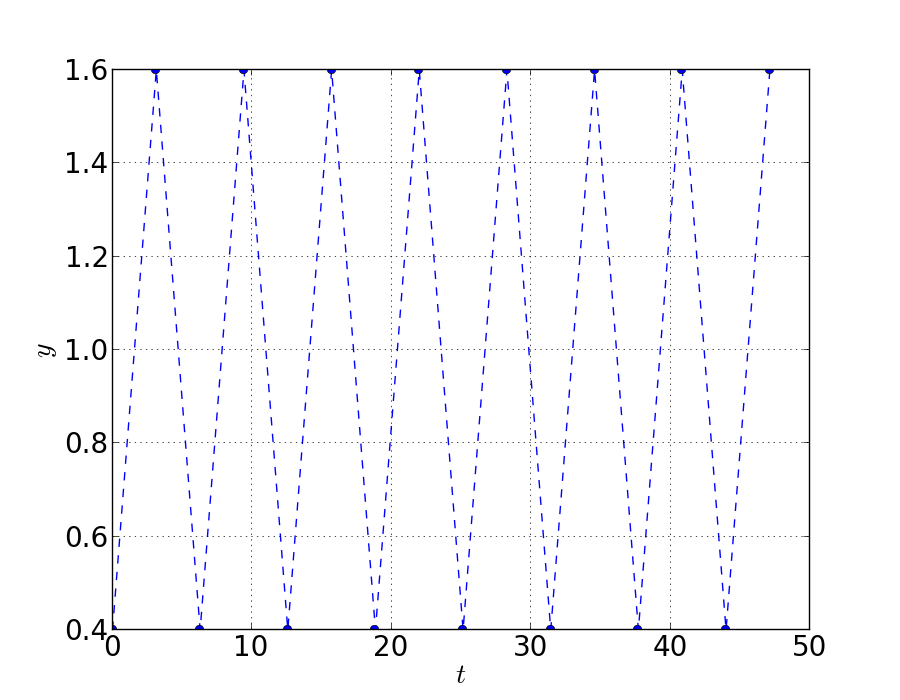
\includegraphics[max size={3 in}{4 in}]{d1.png}
\caption{}
}
\end{figure}

\begin{figure}[H]
\centering{
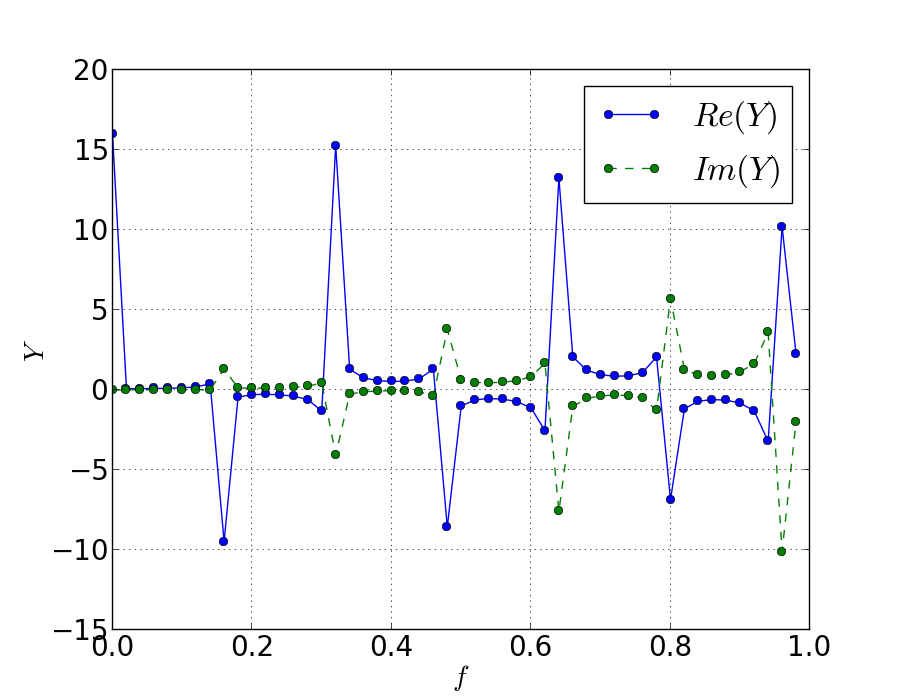
\includegraphics[max size={3 in}{4 in}]{d2.png}
\caption{}
}
\end{figure}

\begin{figure}[H]
\centering{
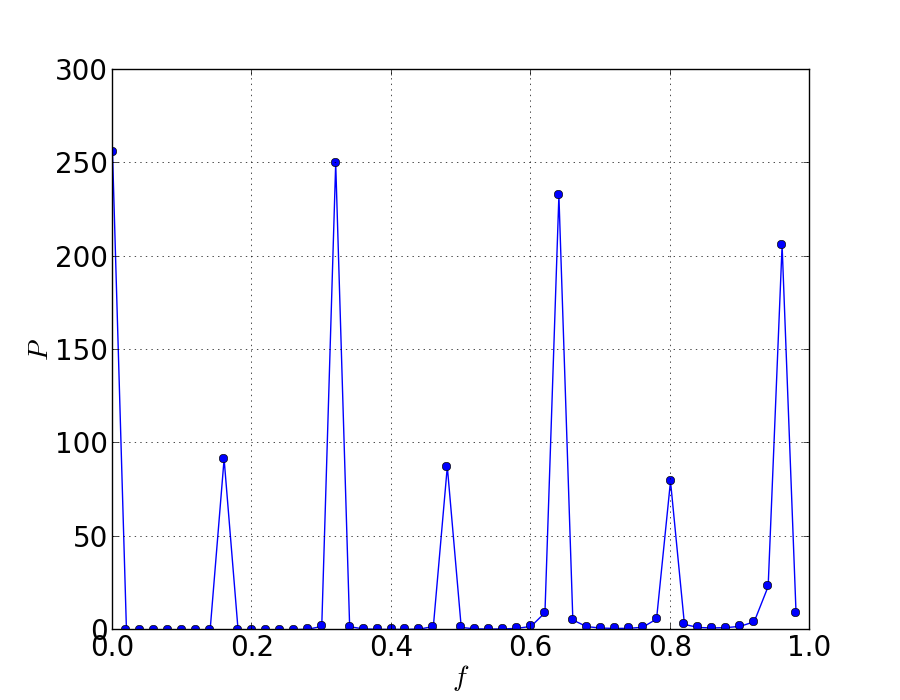
\includegraphics[max size={3 in}{4 in}]{d3.png}
\caption{}
}
\end{figure}

\end{document}